\subsection{Helicopter dynamics}
The magnitude of the thrust generated by each of the rotors is given by the sum of two components, one due to the lift and the other due to the drag. 
\begin{gather*}
    F_l = K_l \omega^2, \\
    F_d = K_d \omega^2,
\end{gather*}
where $\omega$ represents the angular velocity of the rotor, while $K_l$ and $K_r$ are two coefficients, whose expressions are the following:
\begin{gather*}
    K_l = \frac{1}{2} C_l c r^3 \rho, \\
    K_d = \frac{1}{2} C_d c r^3 \rho.
\end{gather*}
In the previous formulas, $c$ is the chord of a rotor blade and $r$ is its hub-to-tip length; $\rho$ is the air density, while $C_l$ and $C_d$ indicate the lift and drag coefficients of the rotor blades, which depend on their angle of attack. We consider the latter constant at a value such that $K_l - K_d > 0$.\\
This means that we can write the total thrust norm generated by each rotor as:
\begin{gather}
    ||F|| = F_l - F_d = (K_l - K_d) \, \omega^2, \label{eq:force_norm}
\end{gather}
therefore we can treat $\omega_u$ and $\omega_l$ as two of the control inputs of the system (respectively, for the upper and lower rotor).

Now consider the angles that the projections of the thrust vectors on the planes $xz$ and $yz$ form with the vertical axis $z$, called respectively $\alpha$ and $\beta$: this couple is the other input of the system, and it is the same for the upper and lower rotors. The two angles are illustrated in Figure \ref{fig:alpha_beta}.

\begin{figure}[H]
    \centering
    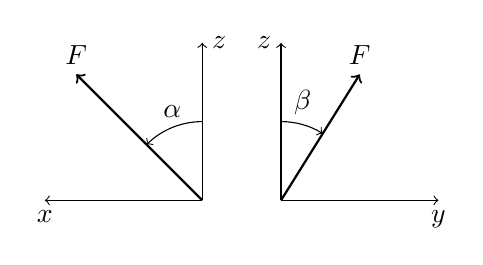
\begin{tikzpicture}[scale=2]
        \draw[->] (0,0) -- (0,1) node[right] {$z$};
        \draw[->] (0,0) -- (-1,0) node[below] {$x$};
        
        \draw[->,thick] (0,0) -- (-0.8,0.8) node[above] {$F$};
        
        \draw[->] (0,0.5) arc (90:135:0.5) node[midway, above] {$\alpha$};

        \draw[->] (0.5,0) -- (0.5,1) node[left] {$z$};
        \draw[->] (0.5,0) -- (1.5,0) node[below] {$y$};
        
        \draw[->,thick] (0.5,0) -- (1,0.8) node[above] {$F$};
        
        \draw[->] (0.5,0.5) arc (90:58:0.5) node[midway, above] {$\beta$};
    \end{tikzpicture}
    \caption{Angles $\alpha$ and $\beta$ that the projections of the thrust vector forms with the vertical direction in the $xz$ and $yz$ planes of the body frame.}
    \label{fig:alpha_beta}
\end{figure}

\noindent In the body reference frame, the thrust vector is then written by means of the auxiliary angle $\gamma$, i.e. the angle that the thrust vector forms with the vertical axis $z$ in the three-dimensional space:
\begin{align}
    F^b = T_{(\alpha, \beta)}||F|| \label{eq:force}
\end{align}
\vspace*{-0.6cm}
\begin{align*}\text{with} \quad T_{(\alpha, \beta)} = \begin{bmatrix}
        -\tan{\alpha} \cos{\gamma} \\
        -\tan{\beta} \cos{\gamma} \\
        \cos{\gamma}
    \end{bmatrix}, \\
    \tan^2{\gamma} = \tan^2{\alpha} + \tan^2{\beta}. 
\end{align*}

Since the thrust vectors are not applied in the center of mass of the helicopter, they also generate torques according to:
\begin{align} 
    \tau^b = \begin{bmatrix}
        0 \\ 0 \\ d_{cm}
    \end{bmatrix} \times F^b, \label{eq:torque_due_force}
\end{align}
with $d_{cm}$ being the distance between the center of mass of the helicopter and the center of the rotors.\\
Note that this cross product results in a vector whose last component is null. In fact, the yaw rotation is caused by the difference of the reaction torques generated by the two rotors:
\begin{align} 
    \tau^b_r = \begin{bmatrix}
        0 \\ 0 \\ Q_u - Q_l
    \end{bmatrix} \quad \text{with} \quad Q = 0.02 \; ||F||. \label{eq:reaction_torque}
\end{align}

According to Newton's second law, the overall force acting on the helicopter is the sum of the forces generated by the two rotors and the force of gravity:
\begin{gather*}
    \begin{split}
        F^b_{tot} & = F^b_u + F^b_l + R^T F^i_g \\
        & = T_{(\alpha, \beta)} (K_l - K_d) (\omega^2_u + \omega^2_l)+ R^T F^i_g,
    \end{split}
\end{gather*}
where \(F^b_{tot}\) is the total force acting on the body and \(F^i_{g}\) is the gravitational force.
Similarly, the total torque is composed of the torques generated by the two rotor thrust vectors (roll and pitch) and the reaction torque of the two rotors (yaw):
\begin{align}
    \tau^b_{tot} = \tau^b_u + \tau^b_l + \tau^b_r,
    \label{eq:torque}
\end{align}
where $\tau_{tot}^b$ is the total torque acting on the body.

By applying these laws, we compute the derivative of the velocity $V$ in the body frame. Neglecting external forces, the cross product term accounts for the Coriolis effect.
This is also done for the angular velocity $\Omega$, where the cross product term represents the gyroscopic effect.
\begin{gather*}
    \frac{d}{dt}{V^b} = \frac{F^b_{tot} - \Omega^b \times (m V^b)}{m}, \\
    \frac{d}{dt}{\Omega^b} = I^{-1} (\tau^b_{tot} - \Omega^b \times (I \Omega^b)).
\end{gather*}
In the inertial frame, the position $P$ and the orientation $W$ of the robot are updated by integrating the velocity and the angular velocity, with:
\begin{gather*}
    \frac{d}{dt}P = R\, V^b, \\ 
    \frac{d}{dt}W = R\, \Omega^b.
\end{gather*}